\documentclass[crop=false]{standalone}

\usepackage[subpreambles=false]{standalone}
\usepackage{import}
\usepackage{graphicx}
\usepackage{subcaption}
\usepackage{tikz}

\begin{document}

\vspace{0.05\linewidth}
\begin{center}
  % \hspace*{-0.08\linewidth}
  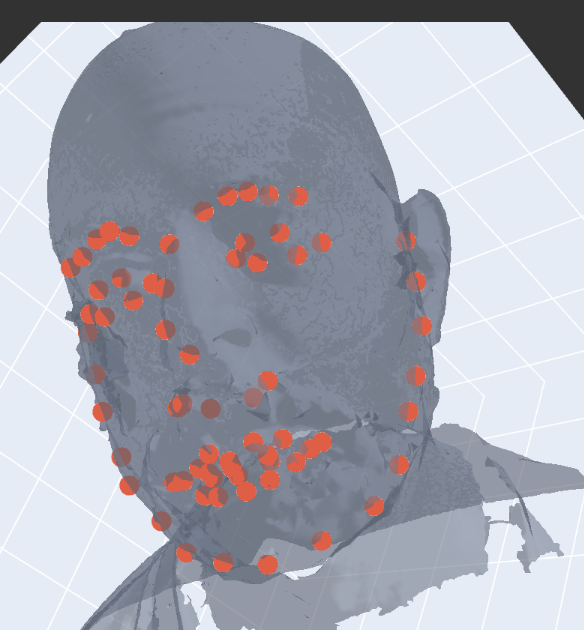
\includegraphics[width=0.4\linewidth]{thesis/appendices/import/imgs/meshcnn_gt.png}
  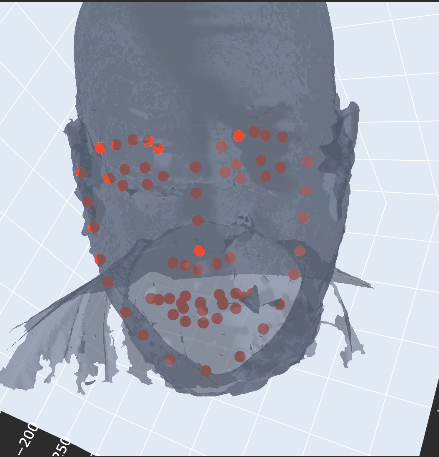
\includegraphics[width=0.4\linewidth]{thesis/appendices/import/imgs/meshcnn_pred.png}
  %\vspace*{-0.06\linewidth}
  \captionof{figure}{
    \textbf{Direct coordinate regression with MeshCNN.}
    \small Left: ground truth. Right: MeshCNN predictions. The overall facial shape is decently captured, but the predictions are very far off. MeshCNN directly operates on the meshes, making it unnecessary perform point sampling. Nonetheless, considerable mesh simplification is required to maintain a manageable memory footprint. Note, that in an earlier version 68 landmarks were processed. However, because most of them are non-anatomical and ill-defined, they were later discarded.
  }
  \label{fig:meshcnn_res}
\end{center}
\vspace{0.05\linewidth}

\end{document}